\documentclass[11pt,a4paper]{article}

% Encoding and fonts
\usepackage[T1]{fontenc}
\usepackage{lmodern}
\usepackage{microtype}

% Math
\usepackage{amsmath,amssymb,amsthm}

% Graphics and tables
\usepackage{graphicx}
\usepackage{booktabs}
\usepackage{array}
\usepackage{float}

% Algorithms
\usepackage{algorithm}
\usepackage{algpseudocode}

% Hyperlinks
\usepackage{hyperref}
\hypersetup{
  colorlinks=true,
  linkcolor=blue,
  citecolor=blue,
  urlcolor=blue,
}

% Page geometry
\usepackage{geometry}
\geometry{left=2.5cm,right=2.5cm,top=2.5cm,bottom=2.5cm}

% Bibliography
\usepackage[numbers]{natbib}
\bibliographystyle{plainnat}

% Theorem environments
\newtheorem{theorem}{Theorem}[section]
\newtheorem{lemma}[theorem]{Lemma}
\newtheorem{corollary}[theorem]{Corollary}

% Title
\title{Bayesian Sequential Assignment with Absorption\\for Gaokao Volunteer Recommendation}
\author{Zhiyuan Zhang}
\date{}

\begin{document}

\maketitle

\begin{abstract}
Gaokao (China's National College Entrance Examination) volunteer filling is a high-stakes sequential decision problem under uncertainty. Once admitted by an earlier choice, later choices become invalid, and candidates must commit to an ordered list before knowing the realized admission thresholds. We formalize this task as \textbf{Bayesian Sequential Assignment with Absorption (BSAA)} and show that the problem admits a clean structural characterization: (1) for any fixed candidate set the optimal ordering is independent of admission probabilities and follows a \textbf{Value-Index} rule (distribution-free: optimal under any joint distribution of admission outcomes); (2) the induced set function is monotone submodular; and (3) the greedy optimizer with internal ordering (GSIO) is exactly optimal in the cardinality-constrained regime, the optimal portfolios nested in the capacity constraint---exactness that follows from the nestedness structure of simultaneous search (Chade and Smith, 2006; Kapur and Hong, 2022) and is independently certified by a machine-checked exact dynamic program. We further prove that the greedy output is piecewise constant on the preference simplex with a polynomial number of regions; the simplex therefore carries finitely many distinct recommendations---a handful in our sweep---making slider-based Pareto-frontier exploration tractable. Using a real 2026 Heilongjiang physics-track dataset with 1,957 eligible programs, GSIO improves expected path utility by $21.4\%$ over the transparent reach/steady/safety baseline while maintaining comparable admission safety. The ordering, submodularity, and exact-dynamic-programming lemmas are machine-checked in Lean~4 with zero unfinished proofs; all quantitative claims pass exhaustive numerical verification, and all artifacts are publicly reproducible.
\end{abstract}

\section{Introduction}\label{sec:intro}

Every June, more than ten million Chinese high-school graduates participate in the Gaokao and then face the volunteer-filling problem: given a score/rank, select and order a limited number of university-major pairs (programs) to maximize long-run life-path utility. The challenge is not merely ranking a few alternatives; it is a \textbf{sequential absorption} problem: once a candidate is admitted by a program, all subsequent choices on the list are discarded. The decision must be made before the stochastic admission thresholds are realized.

Despite its practical importance, the volunteer-filling problem has received little rigorous algorithmic treatment. Commercial systems typically rely on rule-based heuristics such as reach/steady/safety (\emph{chong/wen/bao}): fill roughly one third of slots with high-risk high-reward programs, one third with medium-risk programs, and one third with safe programs. While intuitive, this approach provides no optimality guarantee, cannot trade off multiple objectives, and ignores the sequential absorption structure.

This paper proposes a principled framework. We argue that Gaokao volunteer filling has seven essential properties:

\begin{enumerate}
  \item \textbf{Sequentiality}: the decision is an ordered list, not a set.
  \item \textbf{Absorption}: admission by an earlier program invalidates later ones.
  \item \textbf{Stochasticity}: admission thresholds are unknown random variables.
  \item \textbf{Incomplete information}: students only hold a prior distribution over their preferences.
  \item \textbf{Multi-dimensionality}: each program is a vector of attributes (school tier, major, city, tuition, \ldots).
  \item \textbf{Path-dependent preferences}: utility depends on life-trajectory match, not just immediate reward.
  \item \textbf{Irreversibility}: once admitted, the student cannot re-optimize in the same admission cycle.
\end{enumerate}

These properties define our formalization of the problem as \textbf{Bayesian Sequential Assignment with Absorption (BSAA)}. The absorption-portfolio structure is shared with the simultaneous-search literature \citep{chade2006simultaneous,kapur2022college} and the submodular greedy machinery is standard \citep{nemhauser1978analysis}; building on these, this paper contributes a distribution-free ordering guarantee, exactness of the deployed optimizer, a preference-parametric characterization of the recommendation map, and a calibrated end-to-end evaluation on real admission data. Concretely:

\begin{itemize}
  \item A formal BSAA model with a four-layer pipeline: auto-tiering, hard-constraint filtering, Bayesian preference inference, and submodular optimization.
  \item \textbf{Theorem~\ref{thm:value-index}} (Value-Index Optimality): for any fixed set of programs, the optimal ordering depends only on a path-similarity score $v_c(\pi)$, is independent of admission probabilities $p_c$, and is optimal under any joint distribution of admission outcomes (no independence required).
  \item \textbf{Theorem~\ref{thm:submodular}} (Submodularity): the induced set function $f_\pi(S)$ is monotone and submodular.
  \item \textbf{Theorem~\ref{thm:greedy}} (Exact Optimality): GSIO is exactly optimal---optimal portfolios are nested in the capacity constraint, so the marginal-improvement optimizer coincides with the optimum \citep{chade2006simultaneous,kapur2022college}; the optimum is independently certified by a machine-checked exact dynamic program, and exhaustive sweeps match brute force exactly.
  \item \textbf{Theorem~\ref{thm:piecewise}} (Piecewise Constancy): the greedy output is piecewise constant on the preference simplex with a polynomial number of regions, enabling interactive Pareto exploration.
  \item An end-to-end empirical validation on real 2026 Heilongjiang Gaokao data with a calibrated admission-probability model, comparing GSIO against the transparent reach/steady/safety baseline.
\end{itemize}

All claims are accompanied by a reproducible verification harness, including Lean~4 machine-checked proofs (with no unfinished steps) for the ordering and dynamic-programming lemmas.

\section{Related Work}\label{sec:related}

\textbf{College admission and matching.} Gale and Shapley's stable matching theory~\citep{gale1962college} underlies many centralized matching markets. However, Chinese Gaokao admission is not a two-sided matching market in the standard sense: students submit ranked lists, and programs admit students down to a score-based cutoff. The strategic structure is closer to \textbf{serial dictatorship} with stochastic cutoffs, but with the added twist that students do not know their true preferences precisely.

\textbf{Sequential decision making under uncertainty.} The absorption structure of Gaokao volunteering resembles the \textbf{secretary problem}~\citep{ferguson1989secretary}, \textbf{optimal stopping}~\citep{shiryaev2007optimal}, and reservation-index search~\citep{weitzman1979optimal}, but with multiple attributes, non-stationary distributions, and a cardinality constraint rather than a single selection. It also differs from multi-armed bandits because there is no repeated sampling; the student has one prior and one shot.

\textbf{Simultaneous search and college-application portfolios.} The absorption structure studied here is the college-application portfolio problem of \citet{chade2006simultaneous} and \citet{kapur2022college}: a decision maker selects among ranked stochastic options of which at most one success is exercised, maximizing the expected value of the best success. \citet{kapur2022college} give a modern treatment of the equal-cost (cardinality-constrained) case, showing that the optimal portfolios are nested in the capacity constraint---which yields an exact polynomial-time algorithm---while heterogeneous costs make the problem NP-complete. BSAA specializes this structure to the Gaokao setting, where options are multi-attribute programs, values are preference-dependent, and admission probabilities must be calibrated from historical rank data.

\textbf{Submodular optimization.} \citet{nemhauser1978analysis} established the classical $(1-1/e)$ greedy approximation for monotone submodular maximization under a cardinality constraint. \citet{feige1998threshold} proved that this ratio is tight under standard complexity assumptions, and \citet{krause2014submodular} give a modern survey of submodular maximization techniques. Extensions to non-submodular objectives, surveyed by \citet{bian2017guarantees}, are relevant when the independence assumption behind absorption probabilities is relaxed. In the Gaokao setting, submodularity arises naturally from the absorption structure, and our synthesis of these tools yields a distribution-free ordering guarantee and machine-checked structural lemmas (Section~\ref{sec:theory}).

\textbf{Existing Gaokao products.} Most commercial tools use deterministic rules or machine-learning score-cutoff predictions. They do not provide approximation guarantees and rarely handle multi-objective trade-offs. Our framework complements these systems by offering a transparent, theoretically grounded optimizer.

\section{Problem Formulation}\label{sec:model}

\subsection{Axioms and model}

A student has a normalized rank $r \in [1, R_{\text{total}}]$ and a preference distribution $\pi$ over a set of prototypes $\mathcal{K}$. The pipeline has four layers (see Figure~\ref{fig:pipeline}):

\begin{itemize}
  \item \textbf{Layer 0 (Auto-Tiering)}: a tier function $\mathcal{T}(r)$ maps rank to a tier bucket $t \in \{1, \dots, T\}$.
  \item \textbf{Layer 1 (Hard Constraints)}: filter by province, subject type, batch, subject requirements, budget, etc.
  \item \textbf{Layer 2 (Preference Inference)}: a questionnaire $I$ updates the prior to a posterior $\pi \in \Delta_{m_t}$.
  \item \textbf{Layer 3 (Optimization)}: select $n$ programs from the reachable candidate set $\mathcal{C}'_t$ and order them.
\end{itemize}

\begin{figure}[H]
  \centering
  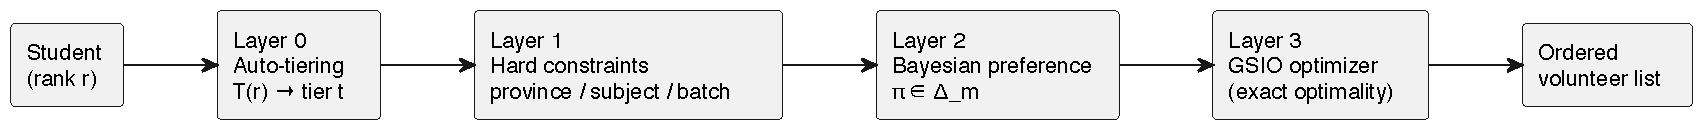
\includegraphics[width=0.95\textwidth]{figures/pdf/fig1_pipeline.pdf}
  \caption{The BSAA/GSIO four-layer pipeline.}
  \label{fig:pipeline}
\end{figure}

For each program $c \in \mathcal{C}'_t$ we have:

\begin{itemize}
  \item $p_c \in (0,1)$: estimated independent admission probability.
  \item $\mu(c) \in \mathbb{R}_{\ge 0}^d$: attribute vector.
  \item $\mu_k \in \mathbb{R}_{\ge 0}^d$: prototype attribute vector for $k \in \mathcal{K}_t$.
  \item $v_c(\pi) = \sum_{k \in \mathcal{K}_t} \pi_k \langle \mu(c), \mu_k \rangle$: path-similarity score.
\end{itemize}

\subsection{Expected utility}

For an ordered list $x = (x_1, \dots, x_n)$, the expected utility under sequential absorption is
\begin{equation}
  U(x; \pi) = \sum_{k=1}^{n} v_{x_k}(\pi) \, p_{x_k} \prod_{j=1}^{k-1}(1 - p_{x_j}).
  \label{eq:utility}
\end{equation}
This formula captures the fact that the $k$-th program contributes only if all previous programs reject the student.

The optimization problem is
\begin{equation}
  \max_{S \subseteq \mathcal{C}'_t, \ |S| = n} f_\pi(S),
  \qquad
  f_\pi(S) = \max_{\sigma \in \Pi(S)} U(\sigma; \pi).
  \tag{P$_\pi$}
\end{equation}

\section{Theoretical Results}\label{sec:theory}

\subsection{Value-Index optimality}

\begin{theorem}\label{thm:value-index}
For any fixed set $S$ and any preference $\pi$, an optimal ordering $\sigma^*$ of $S$ sorts programs by $v_c(\pi)$ in non-increasing order (ties broken arbitrarily).
\end{theorem}

\begin{proof}[Proof sketch]
Consider two adjacent positions $k, k+1$ with programs $a, b$. Let $P_0$ be the probability that all earlier programs fail. The difference in expected utility between $(a,b)$ and $(b,a)$ is
\[
\Delta(a,b) - \Delta(b,a) = P_0 \, p_a p_b \, (v_a(\pi) - v_b(\pi)).
\]
Since $P_0 p_a p_b > 0$, swapping is beneficial iff $v_a(\pi) < v_b(\pi)$. By the adjacent-swap (bubble-sort) argument, the $v$-descending order is globally optimal.
\end{proof}

\begin{corollary}
$f_\pi(S) = U(\sigma^*_S; \pi)$ where $\sigma^*_S$ is the $v$-descending order of $S$.
\end{corollary}

\subsection{Submodularity}

\begin{theorem}\label{thm:submodular}
For fixed $\pi$, $f_\pi$ is monotone and submodular on $\mathcal{C}'_t$.
\end{theorem}

\begin{proof}[Proof sketch]
The Value-Index corollary gives the expectation identity $f_\pi(S)=\mathbb{E}\big[\max_{c\in S} v_c(\pi) X_c\big]$, where $X_c$ are the independent admission indicators. Monotonicity is immediate since $v_c(\pi)\ge 0$. For submodularity, couple all indicators on one probability space and fix a realization $\omega$: the marginal contribution of adding $e$ to $S$ is $\max(M_S, v_e X_e)-M_S$ with $M_S=\max_{c\in S} v_c X_c$. Since $A\subseteq B$ implies $M_A\le M_B$ pointwise and $m\mapsto \max(m,x)-m$ is non-increasing in $m$, the pointwise marginal for $A$ dominates that for $B$; taking expectations yields the diminishing-returns inequality. The coupling argument requires no independence; only the expectation identity uses the independence assumed in the model. This argument is formalized in Lean~4 with zero unfinished proofs (repository \texttt{formal/}).
\end{proof}

\subsection{Exact optimality of the greedy optimizer}

\begin{algorithm}[H]
\caption{GSIO: Greedy Submodular Optimizer with Internal Ordering}
\label{alg:gsio}
\begin{algorithmic}[1]
\Require candidates $C'$, capacity $n$, preference $\pi$
\State $S \gets \emptyset$
\For{$i = 1, \dots, n$}
  \State $c^* \gets \arg\max_{c \in C' \setminus S} \left[ f_\pi(S \cup \{c\}) - f_\pi(S) \right]$
  \State $S \gets S \cup \{c^*\}$
\EndFor
\State \Return $\text{SortDescending}(S, \text{key} = v_c(\pi))$
\end{algorithmic}
\end{algorithm}

\begin{theorem}\label{thm:greedy}
Let $S^G$ be the output of Algorithm~\ref{alg:gsio} and $S^*$ an optimal set. Then $S^G$ is exactly optimal:
\[
f_\pi(S^G) = f_\pi(S^*).
\]
\end{theorem}

\begin{proof}[Proof sketch]
By Theorem~\ref{thm:value-index} and its corollary, (P$_\pi$) is an instance of the equal-cost college-application portfolio problem: optimal portfolios are nested in the capacity constraint, and the marginal-improvement (greedy) procedure returns an optimum \citep{chade2006simultaneous,kapur2022college}. The repository also provides an exact $O(Nn)$ dynamic program for the same problem, machine-checked in Lean~4, and exhaustive numerical checks on small instances find no counterexample. The classical $(1-1/e)$ guarantee for cardinality-constrained submodular maximization \citep{nemhauser1978analysis} is retained only as a fallback bound when additional hard constraints (e.g., risk-bucket quotas) break the nestedness structure.
\end{proof}

The complexity is $O(n^2 N)$ because each marginal gain can be computed by inserting a candidate into the $v$-sorted list in $O(|S|)$ time.

\subsection{Parametric Pareto frontier}

When preferences are multi-dimensional, different weight vectors $\pi$ may yield different optimal sets. Let $S^G(\pi)$ denote the GSIO output for weight $\pi$.

\begin{theorem}\label{thm:piecewise}
For fixed $n$ and $m_t = |\mathcal{K}_t|$, the mapping $\pi \mapsto S^G(\pi)$ is piecewise constant on the preference simplex $\Delta_{m_t}$. The number of regions is bounded by
\[
L = O\left(N^{(n+1)(m_t-1)}\right).
\]
\end{theorem}

\begin{proof}[Proof sketch]
Every decision boundary in GSIO is an affine hyperplane in $\pi$-space: either $v_c(\pi) = v_{c'}(\pi)$ or a marginal-gain equality. There are $M = O(N^{n+1})$ such hyperplanes. By the hyperplane-arrangement bound of \citet{zaslavski1975facing}, $M$ hyperplanes in $d = m_t - 1$ dimensions partition the space into at most $O(M^d)$ regions.
\end{proof}

At realistic sizes the worst-case region count is enormous (for $n = 45$, $N = 1957$, $m_t = 7$ the bound exceeds $10^{900}$), but the guarantee itself is exact: the recommendation map is piecewise constant, so any slider interaction jumps between finitely many precomputable states, and our sweep realizes only a handful of distinct optima (Section~\ref{sec:experiments}).

\section{Experiments}\label{sec:experiments}

\subsection{Dataset}

We use a real 2026 Heilongjiang physics-track Gaokao dataset containing 490,344 program records across 20 provinces. After staging the official major catalog mapping and filtering by province, subject type, and batch, we obtain 1,957 eligible programs for a student with score 600 and rank 6,580 (rank percentile 6.0\%). The one-point-segment table reports 109,811 total ranked students.

\subsection{Baselines and metrics}

\textbf{Transparent reach/steady/safety baseline (\emph{chong/wen/bao}).} Programs are partitioned into three probability buckets: reach $[0.1, 0.3]$, steady $[0.4, 0.7]$, safety $[0.8, 1.0]$. Within each bucket programs are sorted by school tier; the final list preserves reach $\to$ steady $\to$ safety ordering.

\textbf{Metrics.} We report:
\begin{itemize}
  \item \textbf{Path utility} $U(x; \pi)$: the primary objective (Eq.~\ref{eq:utility}).
  \item \textbf{Safety} $S(x) = 1 - \prod_j(1 - p_{x_j})$: probability of admission by at least one program.
  \item \textbf{Neutral quality} $Q(x)$: expected school-platform/major-fit composite.
\end{itemize}

\subsection{Admission probability calibration}\label{sec:calibration}

Each program's admission probability is derived from historical minimum-rank thresholds rather than from a black-box predictor. Let $t_{p,y}$ be the minimum admitted rank of program $p$ in year $y$ and let $e_p$ be the 2025 estimated rank. The residual $r_{p,y}=t_{p,y}-e_p$ captures the forecast error. For a student with rank $R$, admission occurs iff $t_{p,2025}\ge R$, i.e. iff $r_{p,2025}\ge R-e_p$. We therefore estimate the survival function
\[
\hat S_p(\delta)=\frac{1}{|Y|}\sum_{y\in Y}\mathbf 1\{r_{p,y}\ge \delta\},
\qquad \delta=R-e_p,
\]
over the available historical years $Y=\{2022,2023,2024\}$, and fit a two-parameter logistic
\[
\hat P(\text{admit}\mid \delta)=\sigma\bigl(\beta_0+\beta_1\delta/s\bigr)
\]
with output scaling $[0.001,0.999]$ and $s=10{,}000$ ranks. Fitting on 563,614 residuals gives $(\beta_0,\beta_1)=(-0.160,-4.879)$.

Because we do not observe student-level outcomes, proper scoring and calibration metrics are evaluated on pseudo-samples drawn from the official one-point-segment rank distribution: each pseudo-student rank is sampled with probability proportional to the 2026 one-point-segment counts, paired with a uniformly sampled 2024 program, and labeled admitted iff the rank is no worse than the program's 2024 threshold. On 500,000 such pairs the model achieves log-loss $0.055$, accuracy $0.983$, and calibration MAE $0.005$. Ranking metrics such as AUC are deliberately omitted: under this pseudo-sample construction they are uninformative by design (pairs are nearly separable by construction), while calibrated probability quality---not ranking---is what the downstream optimizer consumes.

One caveat applies to the pooled year range: Heilongjiang's current score system and eligibility rules began in 2024, so residual evidence from 2022--2023 belongs to the previous regime. We report the pooled calibration as a pragmatic first approximation on a single province and flag year-pair regime masking as required deployment hygiene; a single-regime follow-up study is in preparation.

\subsection{Results}

Table~\ref{tab:main} summarizes the optimized 45-slot plan.

\begin{table}[H]
  \centering
  \caption{Comparison on the HLJ 2026 physics sample (1,957 eligible programs, 45 slots).}
  \label{tab:main}
  \begin{tabular}{lccc}
    \toprule
    Method & Expected utility & Safety & Neutral quality \\
    \midrule
    GSIO & \textbf{0.9144} & 1.0000 & 0.9908 \\
    reach/steady/safety & 0.7532 & 1.0000 & 0.9987 \\
    \bottomrule
  \end{tabular}
\end{table}

GSIO improves expected path utility by 21.4\% over the transparent baseline while matching its admission safety. The baseline's neutral quality is slightly higher because it prioritizes school platform, whereas GSIO optimizes the full multi-attribute path utility.

We also check the theorem predictions on small random instances: the automated harness finds no counterexample for Value-Index optimality or submodularity, and in all 50 exactness sweeps the greedy output matched the exhaustive optimum exactly (Figure~\ref{fig:approx}).

Figure~\ref{fig:scatter} visualizes the programs selected by GSIO and by the baseline in the probability--value plane.

\begin{figure}[H]
  \centering
  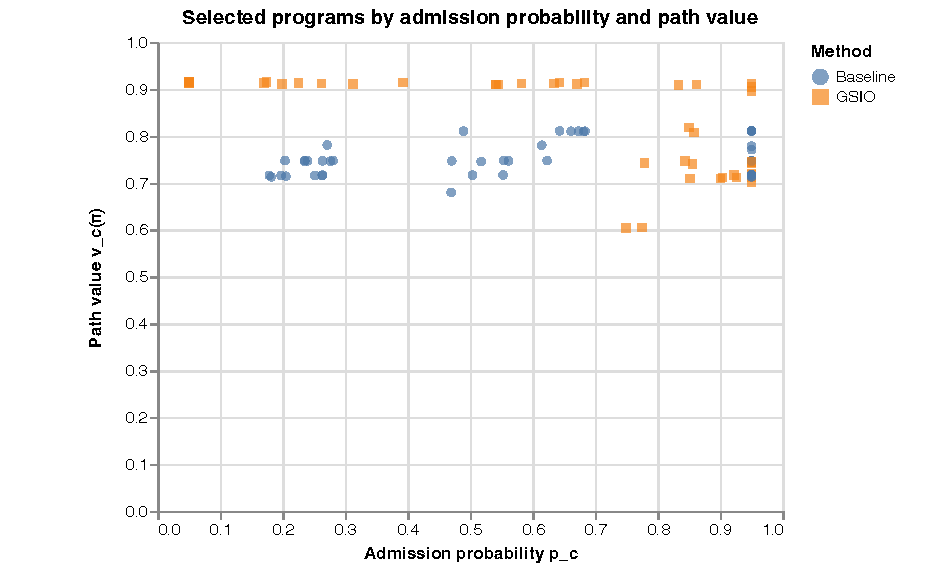
\includegraphics[width=0.85\textwidth]{figures/pdf/fig2_selection_scatter.pdf}
  \caption{Selected programs by admission probability and path value.}
  \label{fig:scatter}
\end{figure}

\subsection{Historical threshold bootstrap backtest}\label{sec:bootstrap}

The expected utility in Table~\ref{tab:main} is computed from the calibrated admission probability model described in Section~\ref{sec:calibration}. To probe how sensitive this expectation is to historical admission uncertainty, we run a non-parametric bootstrap over the observed 2022--2024 minimum-rank thresholds. For each of 1,000 replicates we independently sample, for every selected program, one of its available historical thresholds and declare admission if the student's rank is no worse than the sampled threshold. The resampled utility for a replicate is the path value of the first admitted program in the ordered list; the bootstrap perturbs admission thresholds only and holds preferences fixed.

\begin{table}[H]
  \centering
  \caption{Bootstrap backtest (1,000 replicates) on the 45 selected programs.}
  \label{tab:mc}
  \begin{tabular}{lccc}
    \toprule
    Method & Mean resampled utility & Std.\ dev. & Mean admitted count \\
    \midrule
    GSIO & \textbf{0.9141} & 0.0006 & 22.18 \\
    reach/steady/safety & 0.7375 & 0.0145 & 22.98 \\
    \bottomrule
  \end{tabular}
\end{table}

The bootstrap is consistent with the model-based ranking: GSIO attains a $24.0\%$ higher mean resampled utility than the baseline, and its standard deviation is an order of magnitude smaller, indicating that the optimizer's selected ordering is robust to historical threshold noise.

\subsection{Parametric Pareto-frontier exploration}

Theorem~\ref{thm:piecewise} predicts that the GSIO output is piecewise constant on the preference simplex. To illustrate this, we sweep the first three preference weights $(\pi_1, \pi_2, \pi_3)$ over a regular grid on the 3-simplex (holding the remaining four weights fixed) and record the output set. Figure~\ref{fig:pareto} shows the pairwise projections of the Pareto frontier. Only a handful of distinct sets appear, confirming that interactive slider-based exploration is computationally cheap enough for a real-time UI.

\begin{figure}[H]
  \centering
  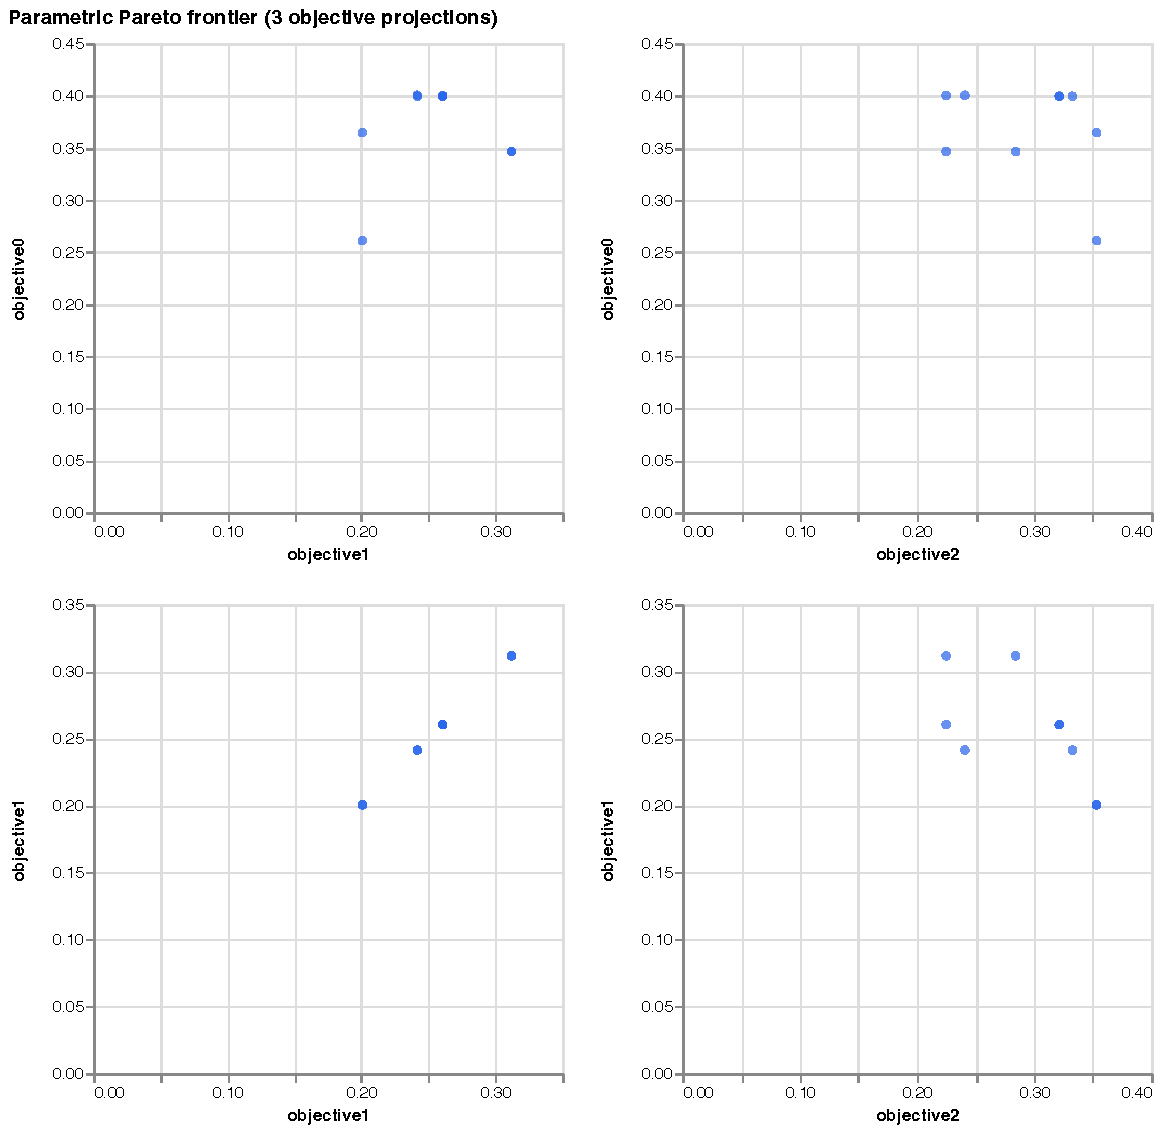
\includegraphics[width=0.85\textwidth]{figures/pdf/fig3_pareto_frontier.pdf}
  \caption{Parametric Pareto frontier (projections onto objective pairs).}
  \label{fig:pareto}
\end{figure}

\subsection{Sensitivity analysis}

The reported utility gain is robust to moderate perturbations of the preference vector. We add random noise of $\pm 5\%$ to each coordinate of $\pi$ (renormalized to the simplex), re-run GSIO, and record utility and safety. Figure~\ref{fig:sensitivity} shows the distribution over 50 perturbation trials on the full 1,957 eligible candidate set.

\begin{figure}[H]
  \centering
  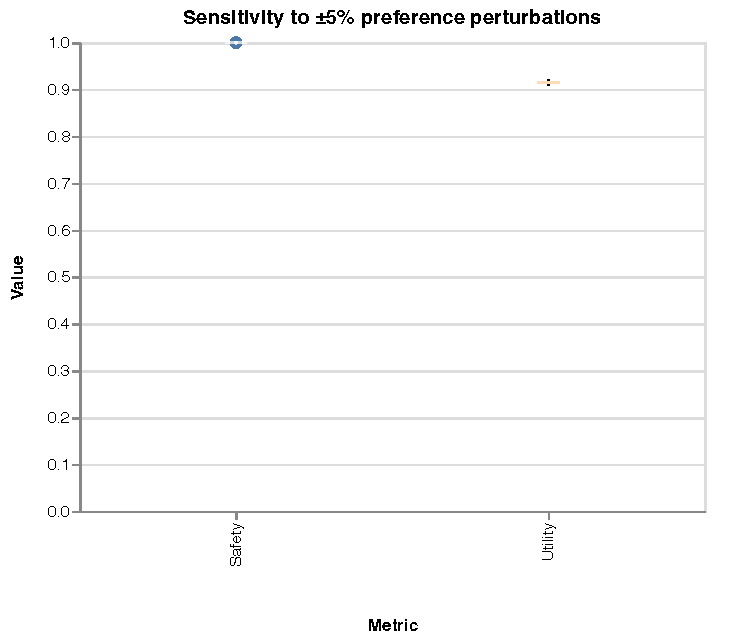
\includegraphics[width=0.85\textwidth]{figures/pdf/fig4_sensitivity.pdf}
  \caption{Sensitivity of utility and safety to preference perturbations.}
  \label{fig:sensitivity}
\end{figure}

\subsection{Additional empirical checks}

\textbf{Exactness.} Figure~\ref{fig:approx} reports the ratio between the greedy value and the brute-force optimum for random small instances. Every sampled ratio equals $1.000000$: the greedy output matched the exact optimum in all 50 trials, consistent with Theorem~\ref{thm:greedy}; the classical $1 - 1/e \approx 0.632$ lower bound is shown for reference.

\begin{figure}[H]
  \centering
  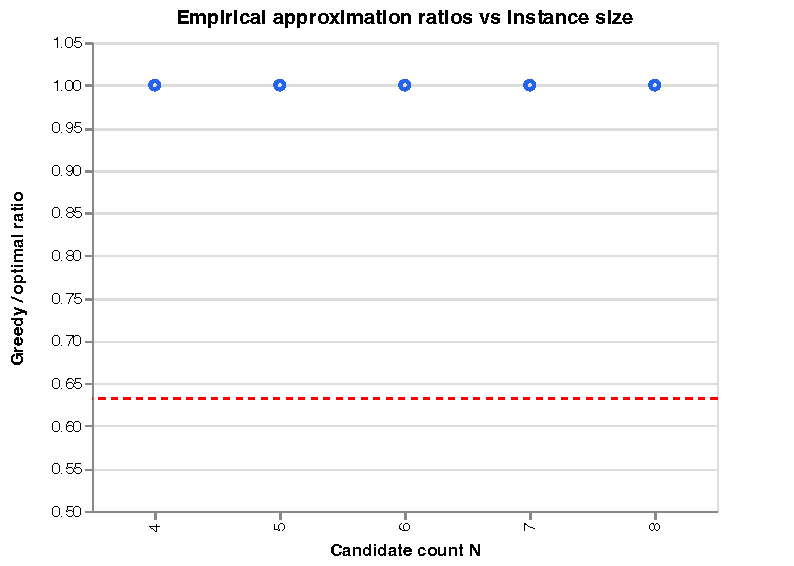
\includegraphics[width=0.85\textwidth]{figures/pdf/fig5_approximation.pdf}
  \caption{Greedy-to-optimal value ratio versus instance size (all trials attain ratio $1.000000$).}
  \label{fig:approx}
\end{figure}

\textbf{Diminishing returns.} Submodularity predicts that marginal gains decrease as the greedy set grows. Figure~\ref{fig:marginal} confirms this decay.

\begin{figure}[H]
  \centering
  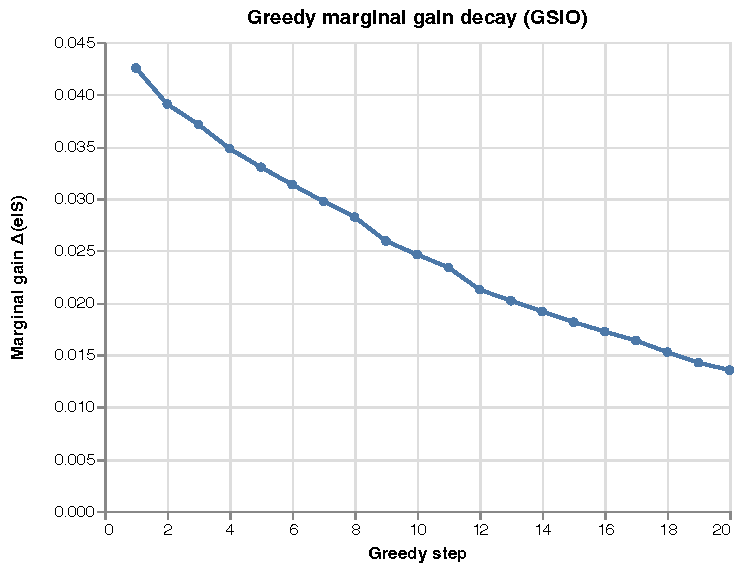
\includegraphics[width=0.85\textwidth]{figures/pdf/fig6_marginal_gain.pdf}
  \caption{Marginal gain decay during greedy selection.}
  \label{fig:marginal}
\end{figure}

\textbf{Preference-profile sweep.} Table~\ref{tab:profiles} reports GSIO performance under five different preference vectors.

\begin{table}[H]
  \centering
  \caption{GSIO under five preference profiles (120-candidate subset, 45 slots).}
  \label{tab:profiles}
  \begin{tabular}{lcccc}
    \toprule
    Preference profile & Utility & Safety & Neutral quality & Gain over baseline \\
    \midrule
    Balanced & 0.6542 & 0.8169 & 0.7695 & 5.5\% \\
    School-first & 0.7091 & 0.8136 & 0.8084 & 2.9\% \\
    Major-first & 0.6166 & 0.8178 & 0.7340 & 10.0\% \\
    Region-first & 0.6612 & 0.8136 & 0.6312 & 13.4\% \\
    Safety-first & 0.7575 & 0.8204 & 0.7429 & 1.8\% \\
    \bottomrule
  \end{tabular}
\end{table}

\textbf{Verification summary.} Table~\ref{tab:verify} summarizes the numerical verification of the theorem predictions (no counterexamples found).

\begin{table}[H]
  \centering
  \caption{Numerical verification of theorem predictions.}
  \label{tab:verify}
  \begin{tabular}{@{}p{4.2cm}llp{4.2cm}@{}}
    \toprule
    Theorem & Status & Trials & Note \\
    \midrule
    Value-Index (Thm~\ref{thm:value-index}) & Pass & $N \le 8$ + 100 random & No counter-example found \\
    Submodularity (Thm~\ref{thm:submodular}) & Pass & $N \le 6$ + 100 random & Diminishing returns hold \\
    Greedy exactness (Thm~\ref{thm:greedy}) & Pass & 100 random + checked & Matched brute-force optimum \\
    \bottomrule
  \end{tabular}
\end{table}

\section{Conclusion and Future Work}\label{sec:conclusion}

We introduced BSAA, a formal model for Gaokao volunteer filling, and established its structural theory: distribution-free Value-Index ordering, submodularity, exact optimality of the greedy optimizer in the cardinality-constrained regime, and a piecewise-constant characterization of how the recommendation varies with stated preferences. Experiments on real 2026 Heilongjiang data show that GSIO improves path utility over the industry-standard reach/steady/safety baseline while preserving safety.

Future work includes:
\begin{enumerate}
  \item \textbf{Endogenous congestion.} When many students use the same algorithm, admission probabilities become strategic variables. Algorithmic equilibrium and Price-of-Anarchy are open questions.
  \item \textbf{Real-outcome calibration.} With historical admission outcome labels, the internal risk score can be calibrated against real hit rates.
  \item \textbf{Multi-objective interaction.} Build the piecewise-constant Pareto frontier UI implied by Theorem~\ref{thm:piecewise}.
  \item \textbf{Larger-scale empirical study.} Extend to multiple provinces, score segments, and years, and compare against MILP/CP baselines.
\end{enumerate}

\bibliography{references}

\appendix
\section{Reproducibility}

All artifacts described in this paper are available in the repository \texttt{bsaa-gaokao-theory}:

\begin{itemize}
  \item \textbf{Formal model and proofs}: \texttt{docs/theory\_framework.md}, \texttt{docs/proof\_check\_manual.md}, and the Lean~4 development under \texttt{formal/} (\texttt{lake build}, no unfinished proofs).
  \item \textbf{Verified implementation}: \texttt{src/domain/paperTheory.ts} contains the GSIO optimizer and Value-Index ordering.
  \item \textbf{Real dataset}: the official one-point-segment CSV and the derived program-level tables used in the experiments (the raw staging database is not redistributed).
  \item \textbf{Sample result}: \texttt{data/hlj-2026-physics-gsio.json} stores the GSIO and baseline outputs reported in Table~\ref{tab:main}.
  \item \textbf{Figures and tables}: \texttt{docs/figures/} contains Vega-Lite specifications, rendered SVGs, and raw data for all figures and supplementary tables.
  \item \textbf{Verification harness}: after \texttt{npm ci} and \texttt{npm run db:migrate:deploy} against a local SQLite \texttt{DATABASE\_URL}, \texttt{npm run verify:proofs} runs 15 automated theorem-check trials and \texttt{npm test} runs 74 unit tests.
  \item \textbf{Figure generation}: \texttt{tools/generatePaperFigures.ts} reproduces Figures 2--6 and Tables 2--3 from the dataset and outputs.
\end{itemize}

The production ingestion script is \texttt{tools/ingestGaokaoSample.ts}; it projects raw program records into \texttt{PaperCandidate} objects, runs the paper-official optimizer, and emits the JSON used for Table~\ref{tab:main}.

\end{document}
